\chapter{Existence of BIBD}

Now lets get back to BIBD and if one exists with parameters $(n,k,\lambda,t)$. Recall that we have steiner triple systems $(n,3,1,2)$ and we can further generalize it to \textbf{Steiner system} which is for $\lambda = 1$; i.e. $(n,k,1,2)$. It is known that $(n,4,1,2)$ and $(n,5,1,2)$ exist non-trivial Steiner system, but for $k > 6$ it is not known.

\begin{thm}[P. Keevash]
	$\forall k, \lambda, t \ \exists n_0$ s.t. BIBD $(n,k,\lambda, t)$ where $n > n_0$ exists \ifft integrality conditions hold. Integrality conditions are the following.
	
	$$
	\lambda \frac{\binom{n - i}{k-i}}{\binom{k-i}{t-i}} \ \text{for all } i \in [t-1] \text{ has to be integers.}
	$$
\end{thm}

\begin{proof}[Proving that integrality conditions are necessary]
	Lets again draw a simple diagram, which can be seen on picture \ref{nec-integr-cond}. Then each such $T$ is in $\lambda$ $M$'s and $M$ is in $\binom{k}{t}$ number of $T$'s. Now lets fix a point $x$ and set $\M' = \{M \in \M; |M \cap X| > 0\}$ and also in the same way $T' = \{T \in \binom{X}{t}; |T \cap X| > 0\}$. And vice versa for all numbers, not just zero.
	
	\begin{figure}[!ht]\centering
		\begin{tikzpicture}
			\draw (0,0) to (6,0);
			\draw (0,3) to (6,3);
			\node (X) at (6.5,0) {$\binom{X}{t}$};
			\node (M) at (6.5,3) {$\M$};
			\draw (2,0) -- (1,3) node[midway, below, left] {$\subseteq$};
			\draw (2,0) -- (2,3);
			\draw (2,0) -- (3,3);
			\node (T) at (2,-.2) {$T$};
			\node (M) at (5,3.2) {$M$};
			
			\draw (3,0) -- (5,3);
			\draw (5,0) -- (5,3);
			\draw (4,0) -- (5,3);
		\end{tikzpicture}
		\caption{Diagram for the proof.}
		\label{nec-integr-cond}
	\end{figure}
\end{proof}

Note that $n_0$ is dependent on all $k,\lambda,t$. So for answering the question if $(k^2 + k +1, k+1, 1, 2)$ exists we cannot do much.

Now consider this following problem. How many blocks (or hyperedges) can you find so that every tuple is in \textbf{at most} $\lambda$ sets? See that we exchanged equality for an inequality.

\begin{defn}
	Lets define a function $m :=$ maximum number of such blocks.
\end{defn}

\begin{thm}[Erd\H os, Hanani]
	$\forall \epsilon \ \exists n_0 \ \forall n \geq n_0$  the following holds
	
	$$
	m(n,k,\lambda,t) \geq \lambda \frac{\binom{n}{k}}{\binom{k}{t}}(1 - \epsilon).
	$$
	\label{existence-of-partial-bibd}
\end{thm}

Erd\H os and Hanani stated this problem and in 1985 V. Rödl solved this problem and proved, that it really holds. He proved it by a method which later on was called Rödl \textbf{nibbling}, which is also essential in Keewash.

\begin{example}
	We have 15 schoolgirls, 7 days in a week and we want to form a groups of 3. Moreover we want that every pair will be together in a group in exactly one day. We may only compute the value
	
	$$
	\frac{\binom{15}{2}}{\binom{3}{2}} = \frac{105}{3} = 35
	$$
	
	\noindent and so it is solvable.
\end{example}

Generally we would like to check if for a hypergraf $(X, \M)$ there exists $\M = \bigcup_i M_i$ where $M_i$ is exactly matching of size $2l+1$.

\section{Conjectures and theorems}

As it was stated before we may furthermore extend the list of conjectures and sometimes even proven theorems.

\begin{topic}{Existence of partial BIBD}
	As it was stated in theorem \ref{existence-of-partial-bibd} for large enough set $X$ there exists such BIBD $(X, \M)$.
\end{topic}

\begin{topic}{Existence of BIBD}
	Furthermore Keewash showed stronger theorem which is about an exsitence of BIBD. The theorem \ref{existence-of-bibd} is stated below.
	
	\begin{thm}[Keewash, Osthus-Kuhn]
		$\exists (X, \M)$ BIBD $(v,k,\lambda,t)$ for every $k,\lambda,t$ and $v \geq v_0 (k,\lambda,t)$ with integrality conditions.
		\label{existence-of-bibd}
	\end{thm}
\end{topic}

\begin{topic}{Ringel tree packing problem}
	We may recall steiner tripple systems in which when we take $K_n$ we want to find edge-disjoint triangles in $K_n$ such that every edge is in one triangle. This problem (and all other similar sounding ones) are typically called \textit{packing problems}. In our special case we know that $|E(K_n)| = \binom{n}{2} = \frac{n}{2} (n-1)$ and in $K_{2n+1}$ we take an arbitrary tree $T$ with $n+1$ vertices. Now the question is if $K_{2n+1}$ can be packed by $2n+1$ copies of $T$.
	
	This was proved as true by Sudakar and Keewash. Also observe that if $|T| = n$ and we would have $K_n$ then having a tree having one vertex with degree $n-1$ it is not possible to pack such tree.
\end{topic}

\begin{topic}{Rosa conjecture}
	Suppose we have a tree $T = (V,E)$ where $|V| = n$/ Does there exist labeling $l : V \to \{1,2, \dots, n\}$ such that $\{|l(v) - l(u)|; \{u,v\} \in E\} = \{1,2, \dots, n-1\}$, i.e. the differences are distinct. This is an \OPEN open problem.
	
	We may not see the relation to the previous topics at a first glance, but imagine having a circle with numbers around it. And we would connect the numbers by edges, which will be corresponding to the labeling, then we would be looking at packing of such model.
\end{topic}

\begin{topic}{Gyarfas}
	Most people will already know that $\binom{n}{2} = \frac{n}{2} (n-1) = 1 + 2 + \dots + (n-1)$ which is well known fact already shown by Gauss. So lets use this to state another packing problem.
	
	Given trees $T_i$ for all $i = 2,3, \dots, n$ where $T_i$ tree has $i-1$ edges (or $i$ vertices). The question is whether such trees packs $K_n$?
	
	\begin{itemize}
		\item When all trees are starts ($T_i$ have one "middle" vertex with degree $i-1$) then it is true. This can be somewhat easily seen.
		\item On the other hand if we have trees which are either of a type star or path it is also true.
		\item But in general it is not known and it is \OPEN open.
	\end{itemize}
\end{topic}

\begin{topic}{Graph dimension}
	Before we state any theorem we must firstly define what is a product of graphs and also dimension of graph.
	
	\begin{defn}[Graph product]
		For graphs $G = (V,E)$ and $G' = (V', E')$ their product $G \times G'$ is defined as a new graph $H = (V \times V', E'')$ where $\{(x,x'),(y,y')\} \in E'' \iff \{x,y\} \in E$ and $\{x',y'\} \in E'$.
	\end{defn}
	
	\begin{figure}[!ht]\centering
		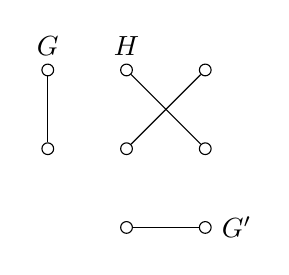
\begin{tikzpicture}[n/.style = {draw, circle, inner sep=1.5pt}]
			\node[n] at (0,1) (1) {};
			\node at (0,2.3) {$G$};
			\node[n] at (0,2) (2) {};
			\node[n] at (1,0) (3) {};
			\node[n] at (2,0) (4) {};
			\node at (2.4,0) {$G'$};
			\draw (1) -- (2);
			\draw (3) -- (4);
			\node[n] at (1,1) (5) {};
			\node[n] at (1,2) (6) {};
			\node[n] at (2,1) (7) {};
			\node[n] at (2,2) (8) {};
			\node at (1,2.3) {$H$};
			\draw (5) -- (8);
			\draw (6) -- (7);
		\end{tikzpicture}
		\caption{Simple example of graph product, where both $G$ and $G'$ are $P_1$.}
	\end{figure}
	
	\begin{defn}[Graph dimension]
		For a graph $G = (V,E)$ we define dimension $\dim(G) = \min(|I|)$ and $G$ is induced subgraph of $\prod_{i \in I} K_{n(i)}$.
	\end{defn}
	
	\begin{thm}
		For every $G$ there exists $n(i); i \in I$ such that $G$ is induced subgraph of $\prod_{i \in I} K_{n(i)}$.
	\end{thm}
	
	\begin{example}
		Lets see some examples of dimensions of graphs, where some may be easier and some harder. Firstly trivially $\dim(K_n) = 1$. Secondly for graph $G$ consisting of a isolated vertex and $K_n$ we have that $\dim(G) = n$. Lastly for a graph $H$ of a matching we get that $\dim(H) = \log n$ which was proved by Lovász, Pultr and Nešetřil.
	\end{example}
	
	When we take a graph $G_{V,1/2}$ which is a random graph with $V$ vertices and every edge has probability $1/2$ that it exists. The lower bound $\dim(G_{V,1/2}) \geq \frac{n}{\log n}$ can be seen by a probabilistic argument and the fact that $\dim(G)$ corresponds to the covering of edges of complement of $G$ by equivalences. Moreover Guo and Warke showed that for constants $c,c'$ we have the following.
	
	$$
	c \frac{n}{\log n} \leq \dim(G_{V,1/2}) \leq c' \frac{n}{\log n}
	$$
\end{topic}

\begin{topic}{Back to STS}
	For STS $(v,3,1,2)$ simple hypergraph $(X, \M)$ where $\M$ contains on $k$ points at least $k-3$ triples; that is for $k \geq 4$. Erd\H os stated if there exists STS $(X, \M)$ such that on any $l$ points there are $\leq l-3$ edges. This was proven as being true.
	
	But what about $|\M| \geq n^{1 + \epsilon}$? This will be shown as being actually hard.
\end{topic}

For simple $k$-graphs $(X, \M)$ we have shown that $\chi$ may be unbounded, due to Ramsey and Hales Jewett, but $PG(g)$ has $\chi = 2$ for $g > 2$. Also $\M \sim \binom{|X|}{2}$ due to Erd\H s and Hanani. Now lets see if $|\M| \geq |X|^{1 + \epsilon}$ can be true. Before showing the proof lets some direct results from such statement.

\begin{thm}[Ordering property]
	Assume $|\M| \geq |X|^{1 + \epsilon}$ fo given $k, \epsilon$ and large $X$. $\forall G = (V,E)$ and $\forall$ linear ordering of $V$ there exists graph $H = (W,F)$ such that for every linear ordering $\preceq$ of $W$ there exist monotone embedding $f : (G, \leq) \to (H, \preceq)$. In particular $f : V \to W$, $\{x,y\} \in E \iff \{f(x), f(y)\} \in F$ and $x \leq y \iff f(x) \preceq f(y)$.
\end{thm}

\begin{proof}
	Let $G = (V,E)$ be given and $|V| = k$. Let $(X, \M)$ be simple $k$-graph with $n$ vertices. Let $\mathcal{G}$ be the set of all graphs $H = (X,F)$ with property that for any $M \in \M$ the graph $H|_M \simeq G$ and every edge of $F$ is a subset of an $M \in \M$. Then the number of placements of different orderings of $G$ is $a = \frac{k!}{\mathtt{Aut}(G)} = a$ where $\mathtt{Aut}(G)$ is the automorfism group of graph $G$.
	
	Then $|\mathcal{G}| = a^{|\M|} \geq a^{n^{1+\epsilon}}$. How many graphs $H$ in $\mathcal{G}$ contain embedding $(G, \leq) \to (H, \preceq)$ for some $\preceq$? That is $\leq n! (a - 1)^{n^{1+\epsilon}}$ which is $\ll a^{n^{1+\epsilon}}$, which can be seen by taking logarithms.
	
	$$
	n^{1 + \epsilon} \log a > n \log n + n^{1 + \epsilon} \log(a-1)
	$$
	
	\noindent Hence there exists $H \ in \mathcal{G}$ such that it suffices the property.
\end{proof}

Other remark is that there exists $H$ where all orderings of $(G, \leq)$ appear almost equally likely, which was shown by Angel, Kechris and Lyons. The technique is called \textit{random placement method} used in 1991 by Nešetřil, Rodl and Ramsey.

Now we will show a stronger version of our stated property.

\begin{thm}
	$\forall k \forall l \exists \epsilon$ There exist $(X, \M)$ $k$-graph such that
	
	\begin{enumerate}
		\item $|\M| \geq |X|^{1 + \epsilon}$ and
		\item $(X, \M)$ has no cycles of length $\leq l$.
	\end{enumerate}
	\label{big-sized-k-graph}
\end{thm}

Note that we can have cycles of length $2$ by just having $M \neq M' \in \M$ where $|M \cap M'| = 2$. This can be seen by drawing the incidence bipartite graph, where we have cycles of length $2l$ in comparison to the circles inside a $k$-graph. Hence for $l = 3$ we obtain the original statement.

\begin{proof}{Proof with stronger theorem.}
	Let $G = (V,E)$ be given and $|V| = k$. Let $(X, \M)$ be simple $k$-graph with $n$ vertices. Let $\mathcal{G}$ be the set of all graphs $H = (X,F)$ with property that for any $M \in \M$ the graph $H|_M \simeq G$ and every edge of $F$ is a subset of an $M \in \M$. Also $H$ contains cycles of length $\leq l$ only in copies of $G$.
\end{proof}

\begin{thm}
	$\forall k \ \forall l \ \exists G_{k,l} = G$:
	
	\begin{enumerate}
		\item $\chi(G) \geq k$ and
		\item $G$ contains no cycles $C_3, C_4, \dots, C_{l-1}$.
	\end{enumerate}
\end{thm}

\begin{proof}
	Put $K = k+1$ and apply stronger theorem \ref{big-sized-k-graph} for $K,l$, then we get $(X, \M)$ $K$-graph and $|X| = n$ and $|\M| \geq |X|^{1 + \epsilon}$. We take $M \in \M$ and we put there one edge. $\mathcal{G} = \{(X,E); (X,E)|_M \simeq \text{only one edge}\}$.
	
	Now $a = \binom{K}{2}$ and any $H \in \mathcal{G}$ does not contain short cycles. How many graphs $H$ in $\mathcal{G}$ have a $\chi(H) \leq k$?
	
	So $\exists f: X \to \{1, 2, \dots, k\}$ on every $M \in \M$ $\exists x \neq y$ such that $f(x) \neq f(y)$. $|\mathcal{G}| = a^{n^{1+\epsilon}} \gg |\{G | \chi(G) \leq k, G \in \mathcal{G}\}| = k^n \cdot (a-1)^{n^{1 + \epsilon}}$.
\end{proof}

Now suppose we have a poset $P = (X, \leq)$ and we create Hase diagram. Question: Which graphs are diagrams? For planar graphs it holds that $G$ is diagram $\iff K_{3} \nsubseteq G \Rightarrow \chi(G) \leq 3$. Problem is that whether there exists graph without $C$ of length $[3, l]$ which fails to be a diagram? Then there is a theorem which states that indeed it is true for all $l$. $G$ is not a diagram $\iff \forall$ ordering $\leq$ of $V(G)$ there exists a cycle of length $t$ for some $t$.

\begin{proof}{Proof of theorem \ref{big-sized-k-graph}}
	Set $\epsilon = \frac{1}{l}$ and put $m = 2 \cdot n^{1+\epsilon}$. Consider all $k$-graphs with $m$ edges and $n$ vertices. There is exactly $\binom{\binom{n}{k}}{m}$ such $k$-graphs. Observe that if $(X, \M)$ has no cycles then $|\M| (k - 1) + 1 \leq |X|$. How many of these $k$-graphs contain a cycle of length $l' \leq l$? By this observation it must be violated so it must be
	
	$$
	\leq c(k, l') n^{(k-1)l'} \binom{\binom{n}{k} - l'}{m - l'}
	$$
	
	\noindent where
	
	$$
	c(k, l') = \binom{\binom{l'(l-1)}{k}}{l'}.
	$$
	
	Lets divide it be $\binom{\binom{n}{k}}{m}$ which leads to upper bound for average number of cycles of length $l'$. So we proceed by summing it over all $l' \leq l$.  Obtaining the following.
	
	$$
	\sum_{l' \leq l} \frac{c(k, l') n^{(k-1)l'} \binom{\binom{n}{k} - l'}{m - l'}}{\binom{\binom{n}{k}}{m}}
	$$
	
	We can simplify the binomials and just obtain
	
	$$
	\frac{m \cdot (m - 1) \cdots 2 \cdot 1}{\binom{n}{k} \cdot (\binom{n}{k} - 1) \cdots (\binom{n}{k} - l' + 1)} \cdot n^{kl' - l'}
	$$
	
	\noindent and we are considering only with going to $\infty$, that is the leading elements of such polynomials. Hence we have
	
	$$
	\leq c \cdot n^{kl' - l'} \cdot \frac{m^{l'}}{n^{kl'}} = c \cdot n^{-l'} \cdot n^{(1 + \epsilon) l'} = c \cdot n^{\epsilon l'} \leq n \cdot c.
	$$
	
	Therefore there has to be $k$-graph with such small number of short cycles. For that we will delete at most $cn$ edges to get rid of every short cycle.
\end{proof}

Note that for this theorem there does not exist a constructive proof.

\begin{cor}
	$\forall p, k \geq 2, l \geq 2$ $\exists (Y, \mathcal{N})$ such that
	
	\begin{enumerate}
		\item $\mathcal{N} \subseteq \binom{Y}{k}$,
		\item $(Y, \mathcal{N})$ has girth $> l$ and
		\item $\chi(Y, \mathcal{N}) > p$.
	\end{enumerate}
	\label{chromatic-girth}
\end{cor}

\begin{proof}
	Put $K = p (k-1) + 1$ and let $(X, \M)$ be simple hypergraph such that $\M \subseteq \binom{X}{K}$ and $(X, \M)$ has girth $> l$ and $|\M| \geq |X|^{1+\epsilon}$ (by using the theorem \ref{big-sized-k-graph}). Let $\mathcal{H}$ be the set of all graphs $(X, \mathcal{N})$, where $\mathcal{N} \subseteq \binom{X}{k}$ such that
	
	\begin{enumerate}
		\item for every $M \in \M$ there exists $\leq 1$ $N \in \mathcal{N}$ where $N \subseteq M$ and
		\item there are no other edges.
	\end{enumerate}
	
	\noindent Any $(X, \mathcal{N}) \in \mathcal{H}$ has girth $> l$. How many $k$-graphs from $\mathcal{H}$ have a chromatic number $< p$? That would be
	
	$$
	\leq p^{|X|} \cdot \left(\binom{K}{k} - 1\right)^{|X|^{1 + \epsilon}}
	$$
	
	\noindent since it is the number of colorings multiplied by the number of $k$-graphs with given coloring (respectively). This is
	
	$$
	\ll |\mathcal{H}| = \left(\binom{K}{k}\right)^{|X|^{1 + \epsilon}}.
	$$
\end{proof}

We will also present a constructive proof in this case. But before we do so, we state some remarks. Usually the \textit{chromatic number} of a graphs is something like the complexity, or in other words it cannot be split into small pieces. On the other hand \textit{girth} is something like local simplicity. So the theorem states that even a graph which locally seems simple it is still complex.

\begin{defn}
	Graph $F$ is $\chi$-unavoidable if $\exists n_0(F)$ for every graph $G$ with $\chi(G) \geq n_0(F)$ contains $F$ as a subgraph (not necessarily induced).
\end{defn}

\begin{cor}
	Forests are only $\chi$-unavoidable graphs.
\end{cor}

\begin{proof}
	If $F$ is not a forest then $F$ has a cycle of length $l$ which by using the theorem \ref{chromatic-girth} can be still made arbitrarily colourful.
	
	Suppose $\chi(G) \gg n_0$ and $F$ is a tree. This implies that $\Delta(G) > n_0$, where $\Delta(G)$ denotes the maximum degree.
	
	Lets have vertices with small degrees and then delete them. Now we may end up with other vertices which now have small degree so we proceed in the same way until we can. After that we take a vertex with the maximum degree this has to have other vertices which also have a high degree and so on, this is how the tree can be constructed.
\end{proof}

\begin{cor}
	$\forall k \ \forall F$ $K$-graph tree $\exists n_0(k,F)$ such that any $\chi(X, \M) \geq n_0$ contains $F$.
\end{cor}

\begin{lemma}
	Any $k$-graph with high chromatic number contains large degree. (Sometimes this is called a sunflower or $\Delta$ system).
\end{lemma}

\begin{proof}
	Suppose $\chi(X, \M) \geq (k-1) \cdot t = n_0$. Then we split vertices into a groups $X_1, X_2, \dots, X_{n_0}$ by their colours. We will take $X_1$ and enlarge it to $X_1'$ as much as possible without violating the colouring. Then for $X_2$ we take $X_2' = X_2 \setminus X_1'$ and again enlarge it. We will continue with all groups. All of them have to be non-empty, otherwise the colouring was not optimal. Lets have $x \in X_{n_0}'$. There has to be an edge to $X_1', X_2', \dots$, because otherwise we would add $x$ to one of them. This is how we got our sunflower.
\end{proof}

\begin{conj}
	Any high chromatic graphs contains either large $K_n$ or given induced tree $T$. Alternatively: Fix $T$ tree, $K_n$. Let $G$ be a graph $K_n \nsubseteq G$ and $T \not\sqsubseteq G$ then $\chi(G) \leq n_0(T, K_n)$.
\end{conj}

\begin{conj}
	Same statement is not true for $k$-graphs.
\end{conj}

\begin{example}
	Lets consider $k = 2$ so graphs and $l = 4$, therefore triangle-free graphs. Try to create $\forall n$ a graph such that $C_3 \nsubseteq G$ and $\chi(G) = n$. For $n = 3$ we take an odd cycle of length 5. Now we can proceed by Mycielski and construct this graph \ref{mycielski}
	
	\begin{figure}[!ht]\centering
		\begin{subfigure}{.45\textwidth}\centering
			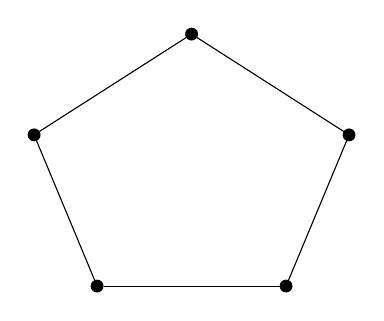
\begin{tikzpicture}[n/.style = {draw, circle, fill, inner sep=1.5pt}, scale=.8]
				\node[n] (0) at (0,0) {};
				\node[n] (1) at (3,0) {};
				\node[n] (2) at (-1,2.4) {};
				\node[n] (3) at (4,2.4) {};
				\node[n] (4) at (1.5,4) {};
				
				\draw (0) -- (1);
				\draw (0) -- (2);
				\draw (3) -- (1);
				\draw (3) -- (4);
				\draw (2) -- (4);
			\end{tikzpicture}
			\caption{Five cycle.}
		\end{subfigure}
		\begin{subfigure}{.45\textwidth}\centering
			\begin{tikzpicture}[n/.style = {draw, circle, fill, inner sep=1.5pt}, scale=.8, b/.style = {myblue, line width=1pt}]
				\node[n] (0) at (0,0) {};
				\node[n] (1) at (3,0) {};
				\node[n] (2) at (-1,2.4) {};
				\node[n] (3) at (4,2.4) {};
				\node[n] (4) at (1.5,4) {};
				
				\node[n,b] (0b) at (0.6,0.6) {};
				\node[n,b] (1b) at (2.4,0.6) {};
				\node[n,b] (2b) at (-0.4,2.4) {};
				\node[n,b] (3b) at (3.4,2.4) {};
				\node[n,b] (4b) at (1.5,3.4) {};
				
				\node[n,b] (c) at (1.5, 2) {};
				
				\draw (0) -- (1);
				\draw (0) -- (2);
				\draw (3) -- (1);
				\draw (3) -- (4);
				\draw (2) -- (4);
				
				\draw[b] (0b) -- (1);
				\draw[b] (0b) -- (2);
				\draw[b] (3b) -- (1);
				\draw[b] (3b) -- (4);
				\draw[b] (2b) -- (4);
				\draw[b] (0) -- (1b);
				\draw[b] (0) -- (2b);
				\draw[b] (3) -- (1b);
				\draw[b] (3) -- (4b);
				\draw[b] (2) -- (4b);
				
				\draw[b] (c) -- (1b);
				\draw[b] (c) -- (2b);
				\draw[b] (c) -- (3b);
				\draw[b] (c) -- (4b);
				\draw[b] (c) -- (0b);
			\end{tikzpicture}
			\caption{Adding brothers and common point.}
		\end{subfigure}
		\caption{Mycielski creation of a graph.}
		\label{mycielski}
	\end{figure}
	
	This can be actually generalized. Lets have $G_n$, for every vertex of such graph create a \textit{"brother"} which will share the same neighbours. Then also create one common vertex and connect all \textit{brothers} to him. See that this has chromatic number at least $n+1$ if $G_n$ had chromatic at least $n$.
\end{example}

\begin{example}
	Another construction is so called \textit{Shift graph.} We will create $G_n$ by taking $V$ to be $E(K_n)$ and $E(G_n)$ being two consecutive edges in $K_n$ by an ordering $\leq$. This graph also does not have triangles and $\chi(G_n) = \log n$. Suppose that $\chi(G_n) \leq t$ then $E = E_1 \dot\cup E_2 \dot\cup \dots \dot\cup E_t = E(K_n)$ easily seen that $\chi([n], E_i) \leq 2$ since no beginnings and ends can overlap. Therefore $\chi(K_n) \leq 2^t$, where the logarithm follows.
\end{example}